
\mode<article>{To apply feedback control, the output $y$ is measured, compared to a desired reference $r$ to give the error signal $e=r-y$. This error is then applied to the control algorithm. If we use a proportional controller (P), the actuator command $x$ is proportional to the error. The gain of the proportional control will be denoted $K_{p}$. }

\begin{frame}{Proportional Control}
\begin{center}
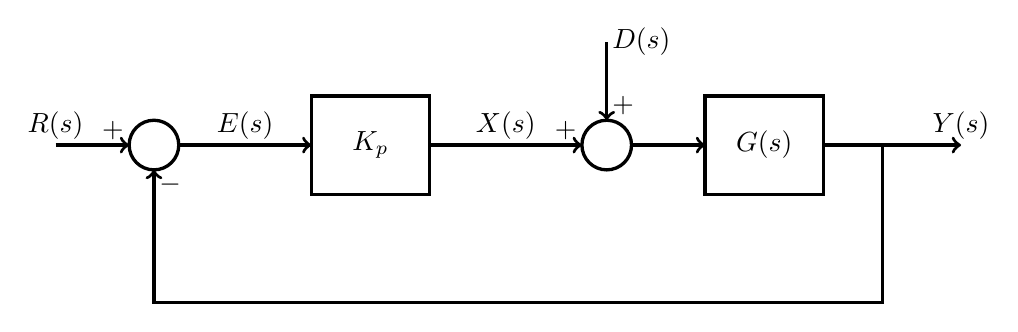
\begin{tikzpicture}[scale=1,inner sep=0pt,outer sep=0pt,very thick,
sysblock/.style={draw,rectangle,inner sep=2pt,minimum width=1.5cm,minimum height=1.25cm,very thick}]

\draw (1.25,0) node[draw,circle] (sum1) {$\rule{0pt}{18pt}$};
\draw (4,0) node[sysblock] (Kp) {$K_{p}$};
\draw (7,0) node[draw,circle] (sum2) {$\rule{0pt}{18pt}$};
\draw (9,0) node[sysblock] (G) {$G(s)$};

\draw[->] (0,0) node[above=2pt] {$R(s)$} -- (sum1.180) node[above left=2pt] {$+$};
\draw[->] (sum1.0) --  node[above=2pt,pos=.5] {$E(s)$} (Kp);
\draw[->] (Kp) -- node[above=2pt,pos=.5] {$X(s)$} (sum2.180) node[above left=2pt] {$+$};
\draw[->] (sum2.0) -- (G);
\draw[->] (G) -- ++(2.5,0) node[above=2pt] {$Y(s)$};
\draw[->] (G) ++(1.5,0) -- ++(0,-2) -| (sum1.-90) node[below right=2pt] {$-$};
\draw[<-] (sum2.90) node[above right=2pt] {$+$} -- ++(0,1) node[right=2pt] {$D(s)$};
\end{tikzpicture}
\end{center}
\end{frame}

When $G(s)$ is a first or second order system, the design of the controller can be straightforward, consisting of three main steps. 
\begin{frame}
\begin{enumerate}
\item \textbf{Collect the design specifications.} Design specifications could be in terms of transient response (rise time, settling time, overshoot) or steady state response (reference tracking or disturbance rejection). 
\item \textbf{Find the relevant {\em closed loop} transfer functions for your design specifications.} \mode<article>{The closed loop transfer functions give the response of the controlled system, as viewed from a reference or disturbance to the output or error. Specifically, using the block diagram simplification rules,}
\begin{align*}
\frac{Y(s)}{R(s)} &= \frac{K_{p}G(s)}{1+K_{p}G(s)}, \\
\frac{E(s)}{R(s)} &= \frac{1}{1+K_{p}G(s)}, \\
\frac{E(s)}{D(s)} &= -\frac{G(s)}{1+K_{p}G(s)}.
\end{align*}
\mode<article>{You will plug the specific open loop transfer function $G(s)$ into these formulas. Note that $\frac{E(s)}{D(s)}$ is only necessary if a disturbance rejection specification is given.}
\item \textbf{Select $K_{p}$ so that the design specifications are met, or determine that no $K_{p}$ exists to meet the specifications.}
\end{enumerate}
\end{frame}

\begin{example}
Design a feedback control system to regulate the height of fluid in a tank, assuming the input flow can be freely assigned. The control system must ensure that the actual tank height follows a reference step command with a settling time $t_{s}\leq 0.2$ s.  In addition, the steady state error between the reference and actual height for a unit step command should be less than or equal to $0.1$. 

A diagram of the feedback control system is below. Note that the output $y$ is the measurement of the tank height $h$. This is subtracted from the reference $r$. The resulting error is multiplied by $K_{p}$ and the flow is set to be this value. The area of the tank is $2$ square meters, the valve constant is $9.81/4$, and the fluid density is $\rho=1$.  

\begin{frame}
\begin{center}
\begin{tikzpicture}
\draw (.75,0) node[above] (tank) {\input{\mainfolder/DrawingElements/FluidElements/tank.tex}};
\draw[decorate,decoration={coil,aspect=0,segment length=5.85pt}] (-.45,2.25) -- ++(2.38,0);
\draw (-1.15,1) node (pipe1) {\input{\mainfolder/DrawingElements/FluidElements/pipe.tex}};
\draw (2.65,1) node (pipe2) {\input{\mainfolder/DrawingElements/FluidElements/valve.tex}};

\draw (1.7,3) node[inner sep=0,outer sep=0] (meas) {\begin{tikzpicture} \draw[very thick] (0,0) -- ++(.1,0) -- ++(0,-.1) -- ++(.2,0) -- ++(0,.1) -- ++(.1,0) -- ++(0,.4) -- ++(-.4,0) -- cycle;\end{tikzpicture}};
\draw (-5.75,1) node[draw,circle,very thick] (sum) {\rule{9pt}{0pt}};
\draw (-4,1) node[draw,rectangle,very thick,minimum width=.5in,minimum height=.5in,outer sep=0pt] (C) {$K_{p}$};

\draw[->,thick,dotted] (meas.90) -- ++(0,.3) node[above left] {measurement of $y=h$} -| (sum.90) node[above right] {$-$};
\draw[<-,thick,dotted] (sum.180) node[above left] {$+$} -- ++(-1,0) node[above] {$r$};
\draw[->,thick,dotted] (sum.0) -- (C.180);
\draw[->,thick,dotted] (C.0) -- ++(.65,0);



\draw[->] (.2,.75) -- node[pos=.5,left] {$h$} ++(0,1.4);
\draw (tank.-90) node{Tank Area: $2$ m$^{2}$};
\draw (pipe2.90) node[above] {$\frac{9.81}{4}$};
\draw (.75,.8) node[above] {$p_{1}$};
\draw[<-] (pipe1.180) ++(.9,0) --  ++(-.5,0) node[left=5pt] {$x=q_{in}$};
\draw[->] (pipe2.0) ++(-.5,0) --  ++(.5,0) node[right] {$q_{out}$};
\draw (.75,2.5) node[above] {$p_{a}$};
\draw (pipe2.0) ++(1.5,0) node {$p_{a}$};
\end{tikzpicture}
\end{center}
\end{frame}

The open loop system transfer function is found using our standard modeling techniques. For example, the following expresses the system as an impedance network with the reference at atmospheric pressure $p_{a}$.

\begin{frame}
\begin{center}
\begin{tikzpicture}
\draw (-2,-1.5) node[scale=.85,inner sep=0pt,outer sep=0pt] (a) {\input{\mainfolder/DrawingElements/CircuitElements/currentsource.tex}};
\draw (-.5,0) node[circle,fill=black,inner sep=0,minimum width=4pt] {} node[above=4pt,circle, inner sep=1pt,fill=yellow] {$P_{1}$};
\draw (a) node[left=9pt] {$Q_{in}(s)$};
\draw (-.5,-1.5) node[rectangle,draw,minimum width=.1in,minimum height=.5in] (tank1) {};
\draw (tank1) node[right=9pt] {$\frac{\rho g}{sA_{1}}$};
\draw (1,0) node[rectangle,draw,minimum width=.5in,minimum height=.1in] (valve1) {};
\draw (valve1) node[above=9pt] {$R_{1}$};
\draw (2.5,-3) node[inner sep=0] (pa) {};
\draw (-.5,-3) node[circle,fill=black,minimum width=4pt,inner sep=0] {};
\draw (-.5,-3) node[below=4pt,circle, inner sep=1pt,fill=pink] {$P_{a}$};
\draw (2.5,-3) node[inner sep=0,outer sep=0] (pa2) {};
\draw (-.5,-3) node[inner sep=0,outer sep=0] (pa3) {};
\draw[very thick] (a.90) |- (valve1.180);
\draw[very thick] (tank1.90) |- (valve1.180);
\draw[very thick] (valve1.0) -| (pa) -- (pa3);
\draw[very thick] (tank1.-90) -- (pa3) -| (a.-90);
\draw[->] (3,-1) -- node[pos=.5,right] {$Q_{out}(s)$} ++(0,-1);
\end{tikzpicture}
\mode<presentation>{\[
\frac{Q_{out}(s)}{Q_{in}(s)} = \frac{\frac{1}{2}}{s+2}
\]}
\end{center}
\end{frame}
We also have the auxiliary equation $\rho g h = p_{1}$, or since $\rho=1$, $h=\frac{1}{g}p_{1}$. Thus, the transfer function $H(s)/Q_{in}(s)$ can be found by first finding $P_{1}/Q_{in}(s)$, and then dividing by $g$. Combining the impedances in parallel, 
\begin{align*}
\frac{P_{1}}{Q_{in}(s)}&= \frac{\frac{g}{2s}\frac{9.81}{4}}{\frac{g}{2s} + \frac{9.81}{4}} \\
 &= \frac{\frac{g}{2}}{\frac{2g}{9.81} + s} 
\end{align*}
Using $g=9.81$ and $h=\frac{1}{g}p_{1}$
\[
G(s) = \frac{H(s)}{Q_{in}(s)} = \frac{\frac{1}{2}}{s+2}
\]

The feedback control system can be represented with the following block diagram. (Since no disturbance rejection specification was listed, a disturbance input was not included.) Note that $R(s)$ is the {\em desired} tank height.

\begin{frame}
\begin{center}
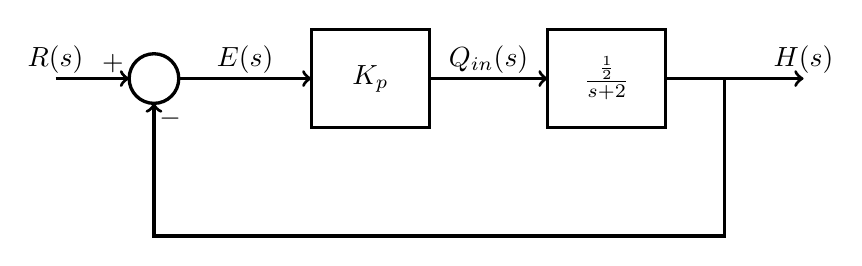
\begin{tikzpicture}[scale=1,inner sep=0pt,outer sep=0pt,very thick,
sysblock/.style={draw,rectangle,inner sep=2pt,minimum width=1.5cm,minimum height=1.25cm,very thick}]

\draw (1.25,0) node[draw,circle] (sum1) {$\rule{0pt}{18pt}$};
\draw (4,0) node[sysblock] (Kp) {$K_{p}$};
\draw (7,0) node[sysblock] (G) {$\frac{\frac{1}{2}}{s+2}$};

\draw[->] (0,0) node[above=2pt] {$R(s)$} -- (sum1.180) node[above left=2pt] {$+$};
\draw[->] (sum1.0) --  node[above=2pt,pos=.5] {$E(s)$} (Kp);
\draw[->] (Kp) -- node[above=2pt] {$Q_{in}(s)$} (G);
\draw[->] (G) -- ++(2.5,0) node[above=2pt] {$H(s)$};
\draw[->] (G) ++(1.5,0) -- ++(0,-2) -| (sum1.-90) node[below right=2pt] {$-$};
\end{tikzpicture}
\end{center}
\end{frame}

We can now proceed with the design process:

\begin{frame}
\begin{enumerate}
\item Design specifications
\begin{itemize}
\item $\ts \leq 0.2$ s
\item $e_{ss}\leq 0.1$ for unit step reference
\end{itemize}
\item Closed loop transfer functions
\begin{align*}
\frac{H(s)}{R(s)} &= \frac{K_{p}/2}{s+\frac{K_{p}}{2}+2}\\
\frac{E(s)}{R(s)} &= \frac{s+2}{s+\frac{K_{p}}{2}+2}\\ 
\end{align*}
Note that the closed loop transfer functions are also first order.
\end{enumerate}
\end{frame}
\begin{frame}
\mode<presentation>{
\begin{center}
$\frac{H(s)}{R(s)} = \frac{K_{p}/2}{s+\frac{K_{p}}{2}+2} \quad \frac{E(s)}{R(s)} = \frac{s+2}{s+\frac{K_{p}}{2}+2}$
\end{center}
}
\begin{enumerate}
\setcounter{enumi}{1}
\item Select $K_{p}$. 
\mode<presentation>{
\begin{itemize}
\item<2-> $\ts \leq 0.2$. 
\[
\ts = \tseqone \leq 0.2 \implies \sigma \geq \frac{4.6}{0.2} = 23
\]
\[
\uncover<3->{\sigma = \frac{K_{p}}{2}+2 \geq 23 \implies K_{p} \geq 42}
\]
\item<4-> $e_{ss}\leq 0.1$.
\[
e_{ss} = \lim_{s\rightarrow 0} s E(s) = \lim_{s\rightarrow 0} s \frac{E(s)}{R(s)}\frac{1}{s} =  s\frac{s+2}{s+\frac{K_{p}}{2}+2}\frac{1}{s} = \frac{2}{2+\frac{K_{p}}{2}} 
\]
\[
\uncover<5->{e_{ss}= \frac{2}{2+\frac{K_{p}}{2}} \leq 0.1 \implies K_{p} \geq 36}
\]
\end{itemize}
}
\mode<article>{We have two specifications. The first constraint on settling time can be converted to a constraint on the closed loop pole location. We previously showed that for a first order system with pole at $s=-\sigma$,
\[
\ts = \tseqone
\]
Since our specification is $t_{s}\leq 0.2$, we require $\frac{4.6}{\sigma}\leq 0.2$ or
\[
\sigma \geq \frac{4.6}{0.2} = 23
\]
The pole of our closed loop feedback system is at $s=-(\frac{K_{p}}{2}+2)$. Thus, we need to choose
\[
\frac{K_{p}}{2}+2 \geq 23
\]
or
\[
K_{p} \geq 42.
\]
The second constraint on reference steady state error translates to a constraint on the DC gain of $K_{p}G(s)$. We can either recall that for a step reference $e_{ss}=\frac{1}{1+K_{s}}$ where $K_{s} = K_{p}G(0) = \frac{K_{p}}{4}$, or we can solve directly using the final value theorem
\[
e_{ss} = \lim_{s\rightarrow 0} s E(s) = \lim_{s\rightarrow 0} s \frac{s+2}{s+\frac{K_{p}}{2}+2}\frac{1}{s} = \frac{2}{2+\frac{K_{p}}{2}} =\frac{1}{1+\frac{K_{p}}{4}}
\]
Since we require
\[
e_{ss} = \frac{1}{1+\frac{K_{p}}{4}} \leq 0.1,
\]
we can solve for the constraint
\[
K_{p} \geq 36
\]
Since the most stringent requirement is on the settling time, our final design choice is
\[
\boxed{K_{p} \geq 42}
\]}
\end{enumerate}
\end{frame}

\end{example}


\begin{example} Determine how a proportional feedback control system will change the closed loop behavior when controlling the position of the mass-spring-damper system using force actuation
\begin{frame}
\begin{center}
\begin{tikzpicture}[scale=1.75,inner sep=0pt,outer sep=0pt,very thick]
\draw (.3,0) node[fill] (a) {}; 
\draw (1.7,0) node[fill] (b) {};
 
\draw (0,0) node (gnd1) {\input{\mainfolder/DrawingElements/MechanicalElements/ground.tex}};
\draw (1,.3) node (K1) {\begin{tikzpicture}
\draw (.75,0) node[inner sep=0,outer sep=0] (K1) {\begin{tikzpicture}
\draw (.75,0) node[inner sep=0,outer sep=0] (K1) {\begin{tikzpicture}
\draw (.75,0) node[inner sep=0,outer sep=0] (K1) {\input{\mainfolder/DrawingElements/MechanicalElements/spring.tex}};
\draw (K1)  node[above=6pt] {$k$};
\draw[very thick] (K1.180) -- ++(-.2,0);
\draw[very thick] (K1.0) -- ++(0.2,0);
\draw[<-,thick] (K1.0) ++(.2,0) -- ++(.5,0) node[right] {$f$};
\draw[<-,thick] (K1.180) ++(-.2,0) -- ++(-.5,0) node[left] {$f$};
\draw[|->,thick] (K1.180) ++(-.2,.4) node[above=2pt] {$x_{1}$} -- ++(.5,0);  
\draw[|->,thick] (K1.0) ++(.2,.4) node[above=2pt] {$x_{2}$} -- ++(.5,0);  
\draw<2-> (K1) ++(0,-.6) node {$f=k(x_{1}-x_{2})$};
\end{tikzpicture}
};
\draw (K1)  node[above=6pt] {$k$};
\draw[very thick] (K1.180) -- ++(-.2,0);
\draw[very thick] (K1.0) -- ++(0.2,0);
\draw[<-,thick] (K1.0) ++(.2,0) -- ++(.5,0) node[right] {$f$};
\draw[<-,thick] (K1.180) ++(-.2,0) -- ++(-.5,0) node[left] {$f$};
\draw[|->,thick] (K1.180) ++(-.2,.4) node[above=2pt] {$x_{1}$} -- ++(.5,0);  
\draw[|->,thick] (K1.0) ++(.2,.4) node[above=2pt] {$x_{2}$} -- ++(.5,0);  
\draw<2-> (K1) ++(0,-.6) node {$f=k(x_{1}-x_{2})$};
\end{tikzpicture}
};
\draw (K1)  node[above=6pt] {$k$};
\draw[very thick] (K1.180) -- ++(-.2,0);
\draw[very thick] (K1.0) -- ++(0.2,0);
\draw[<-,thick] (K1.0) ++(.2,0) -- ++(.5,0) node[right] {$f$};
\draw[<-,thick] (K1.180) ++(-.2,0) -- ++(-.5,0) node[left] {$f$};
\draw[|->,thick] (K1.180) ++(-.2,.4) node[above=2pt] {$x_{1}$} -- ++(.5,0);  
\draw[|->,thick] (K1.0) ++(.2,.4) node[above=2pt] {$x_{2}$} -- ++(.5,0);  
\draw<2-> (K1) ++(0,-.6) node {$f=k(x_{1}-x_{2})$};
\end{tikzpicture}
};
\draw (1,.3) node[above=.2in] {$k$};
\draw (1,-.3) node (D) {\begin{tikzpicture}
\draw[very thick] (-.2,0) -- (0,0);
\draw (.75,0) node {\begin{tikzpicture}
\draw[very thick] (-.2,0) -- (0,0);
\draw (.75,0) node {\begin{tikzpicture}
\draw[very thick] (-.2,0) -- (0,0);
\draw (.75,0) node {\input{\mainfolder/DrawingElements/MechanicalElements/damper.tex}};
\draw (.75,0) node[above=9pt] {$b$};
\draw[very thick] (1.5,0) -- ++(.2,0);
    \draw[<-,thick] (1.5,0) ++(.2,0) -- ++(.5,0) node[right] {$f$};
    \draw[<-,thick] (-.2,0) -- ++(-.5,0) node[left] {$f$};
    \draw[|->,thick] (-.2,.4) node[above=2pt] {$x_{1}$} -- ++(.5,0);  
    \draw[|->,thick] (1.7,.4) node[above=2pt] {$x_{2}$} -- ++(.5,0);  
    \draw (.6,-.6) node {$x=x_{1}-x_{2}$};
  %  \draw (.6,-1.2) node {$f=b\dot{x}$};
\end{tikzpicture}};
\draw (.75,0) node[above=9pt] {$b$};
\draw[very thick] (1.5,0) -- ++(.2,0);
    \draw[<-,thick] (1.5,0) ++(.2,0) -- ++(.5,0) node[right] {$f$};
    \draw[<-,thick] (-.2,0) -- ++(-.5,0) node[left] {$f$};
    \draw[|->,thick] (-.2,.4) node[above=2pt] {$x_{1}$} -- ++(.5,0);  
    \draw[|->,thick] (1.7,.4) node[above=2pt] {$x_{2}$} -- ++(.5,0);  
    \draw (.6,-.6) node {$x=x_{1}-x_{2}$};
  %  \draw (.6,-1.2) node {$f=b\dot{x}$};
\end{tikzpicture}};
\draw (.75,0) node[above=9pt] {$b$};
\draw[very thick] (1.5,0) -- ++(.2,0);
    \draw[<-,thick] (1.5,0) ++(.2,0) -- ++(.5,0) node[right] {$f$};
    \draw[<-,thick] (-.2,0) -- ++(-.5,0) node[left] {$f$};
    \draw[|->,thick] (-.2,.4) node[above=2pt] {$x_{1}$} -- ++(.5,0);  
    \draw[|->,thick] (1.7,.4) node[above=2pt] {$x_{2}$} -- ++(.5,0);  
    \draw (.6,-.6) node {$x=x_{1}-x_{2}$};
  %  \draw (.6,-1.2) node {$f=b\dot{x}$};
\end{tikzpicture}};
\draw (1,-.3) node[below=.22in] {$b$};
\draw (2.5,0) node (M1) {\input{\mainfolder/DrawingElements/MechanicalElements/mass2.tex}};
\draw (2.5,0) node {$m$};
\draw[|->] (2.5,.8) node[above=.15in] {$y$} -- ++(.5,0);


\draw (gnd1) -- (a);
\draw (a) |- (K1);
\draw (a) |- (D);
\draw (K1) -| (b);
\draw (D) -| (b);
\draw (b) -- (M1);
%\draw[->] (M1.0) ++(0,.4) -- ++(.5,0) node[right] {$d$};
\draw[->] (M1.0) -- ++(.5,0) node[right] {$f$};

\end{tikzpicture}
\end{center}
\[
\frac{Y(s)}{F(s)} = \frac{1/m}{s^{2}+(b/m)s + (k/m)}
\]
\end{frame}

The proportional feedback control system would be represented by the block diagram
\begin{frame}
\begin{center}
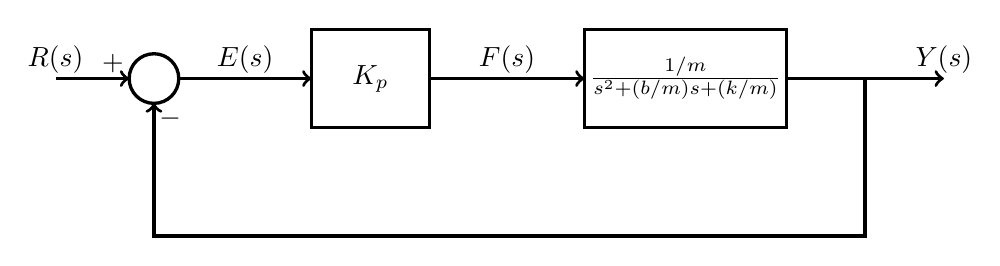
\begin{tikzpicture}[scale=1,inner sep=0pt,outer sep=0pt,very thick,
sysblock/.style={draw,rectangle,inner sep=2pt,minimum width=1.5cm,minimum height=1.25cm,very thick}]

\draw (1.25,0) node[draw,circle] (sum1) {$\rule{0pt}{18pt}$};
\draw (4,0) node[sysblock] (Kp) {$K_{p}$};
\draw (8,0) node[sysblock] (G) {$\frac{1/m}{s^{2}+(b/m)s + (k/m)}$};

\draw[->] (0,0) node[above=2pt] {$R(s)$} -- (sum1.180) node[above left=2pt] {$+$};
\draw[->] (sum1.0) --  node[above=2pt,pos=.5] {$E(s)$} (Kp);
\draw[->] (Kp) -- node[above=2pt, pos=.5] {$F(s)$} (G);
\draw[->] (G.0) -- ++(2,0) node[above=2pt] {$Y(s)$};
\draw[->] (G.0) ++(1,0) -- ++(0,-2) -| (sum1.-90) node[below right=2pt] {$-$};
\end{tikzpicture}
\mode<presentation>{
\[
F(s) = K_{p}(R(s) - Y(s))
\]
\[
f(t) = K_{p}(r(t) - y(t))
\]
}
\end{center}
\end{frame}



The closed loop transfer function is
\begin{frame}
\[
\frac{Y(s)}{R(s)} = \frac{K_{p}/m}{s^{2}+(b/m)s+(k+K_{p})/m}.
\]

\mode<article>{We can get a very general sense of how changes in $K_{p}$ affect the transient response by finding the damping ratio and natural frequency for the closed loop poles. In particular}
\visible<2->{\[\omega_{n} = \sqrt{\frac{k+K_{p}}{m}}, \quad
\zeta  = \frac{b}{2\sqrt{m}\sqrt{k+K_{p}}}, \quad
\zeta\omega_{n}  = \frac{b}{2m}. 
\]}

\mode<article>{From the form of these equations we see that} 
\visible<3->{\begin{align*}
\uparrow K_{p} \implies\begin{cases} \uparrow  \omega_{n} & \implies \mbox{reduced rise time}\\
 \downarrow\zeta & \implies \mbox{increased overshoot} \\
\leftrightarrow \ts & \implies \mbox{no change in settling time} \end{cases}
\end{align*}}
\end{frame}
Thus, while increasing $K_{p}$ makes the response faster, it also makes it more oscillatory, and in the second order case, proportional control cannot change the settling time.

\end{example}

A physical intuition for the behavior of proportional control on a second order system can be obtained by implementing proportional control using a {\em mechanical} controller. Note that in proportional control, the control force $f$ should be given by 
\[
f(t) = K_{p}(r(t)-y(t)).
\]
Let's implement this force by attaching a spring with spring constant $K_{p}$ with one end on the mass, and the other end attached to a point that specifies the reference $r$, as follows:
\begin{frame}
\begin{center}
\begin{tikzpicture}[scale=1.75,inner sep=0pt,outer sep=0pt,very thick]
\draw (.3,0) node[fill] (a) {}; 
\draw (1.7,0) node[fill] (b) {};
 
\draw (0,0) node (gnd1) {\input{\mainfolder/DrawingElements/MechanicalElements/ground.tex}};
\draw (1,.3) node (K1) {\begin{tikzpicture}
\draw (.75,0) node[inner sep=0,outer sep=0] (K1) {\begin{tikzpicture}
\draw (.75,0) node[inner sep=0,outer sep=0] (K1) {\begin{tikzpicture}
\draw (.75,0) node[inner sep=0,outer sep=0] (K1) {\input{\mainfolder/DrawingElements/MechanicalElements/spring.tex}};
\draw (K1)  node[above=6pt] {$k$};
\draw[very thick] (K1.180) -- ++(-.2,0);
\draw[very thick] (K1.0) -- ++(0.2,0);
\draw[<-,thick] (K1.0) ++(.2,0) -- ++(.5,0) node[right] {$f$};
\draw[<-,thick] (K1.180) ++(-.2,0) -- ++(-.5,0) node[left] {$f$};
\draw[|->,thick] (K1.180) ++(-.2,.4) node[above=2pt] {$x_{1}$} -- ++(.5,0);  
\draw[|->,thick] (K1.0) ++(.2,.4) node[above=2pt] {$x_{2}$} -- ++(.5,0);  
\draw<2-> (K1) ++(0,-.6) node {$f=k(x_{1}-x_{2})$};
\end{tikzpicture}
};
\draw (K1)  node[above=6pt] {$k$};
\draw[very thick] (K1.180) -- ++(-.2,0);
\draw[very thick] (K1.0) -- ++(0.2,0);
\draw[<-,thick] (K1.0) ++(.2,0) -- ++(.5,0) node[right] {$f$};
\draw[<-,thick] (K1.180) ++(-.2,0) -- ++(-.5,0) node[left] {$f$};
\draw[|->,thick] (K1.180) ++(-.2,.4) node[above=2pt] {$x_{1}$} -- ++(.5,0);  
\draw[|->,thick] (K1.0) ++(.2,.4) node[above=2pt] {$x_{2}$} -- ++(.5,0);  
\draw<2-> (K1) ++(0,-.6) node {$f=k(x_{1}-x_{2})$};
\end{tikzpicture}
};
\draw (K1)  node[above=6pt] {$k$};
\draw[very thick] (K1.180) -- ++(-.2,0);
\draw[very thick] (K1.0) -- ++(0.2,0);
\draw[<-,thick] (K1.0) ++(.2,0) -- ++(.5,0) node[right] {$f$};
\draw[<-,thick] (K1.180) ++(-.2,0) -- ++(-.5,0) node[left] {$f$};
\draw[|->,thick] (K1.180) ++(-.2,.4) node[above=2pt] {$x_{1}$} -- ++(.5,0);  
\draw[|->,thick] (K1.0) ++(.2,.4) node[above=2pt] {$x_{2}$} -- ++(.5,0);  
\draw<2-> (K1) ++(0,-.6) node {$f=k(x_{1}-x_{2})$};
\end{tikzpicture}
};
\draw (1,.3) node[above=.2in] {$k$};
\draw (1,-.3) node (D) {\begin{tikzpicture}
\draw[very thick] (-.2,0) -- (0,0);
\draw (.75,0) node {\begin{tikzpicture}
\draw[very thick] (-.2,0) -- (0,0);
\draw (.75,0) node {\begin{tikzpicture}
\draw[very thick] (-.2,0) -- (0,0);
\draw (.75,0) node {\input{\mainfolder/DrawingElements/MechanicalElements/damper.tex}};
\draw (.75,0) node[above=9pt] {$b$};
\draw[very thick] (1.5,0) -- ++(.2,0);
    \draw[<-,thick] (1.5,0) ++(.2,0) -- ++(.5,0) node[right] {$f$};
    \draw[<-,thick] (-.2,0) -- ++(-.5,0) node[left] {$f$};
    \draw[|->,thick] (-.2,.4) node[above=2pt] {$x_{1}$} -- ++(.5,0);  
    \draw[|->,thick] (1.7,.4) node[above=2pt] {$x_{2}$} -- ++(.5,0);  
    \draw (.6,-.6) node {$x=x_{1}-x_{2}$};
  %  \draw (.6,-1.2) node {$f=b\dot{x}$};
\end{tikzpicture}};
\draw (.75,0) node[above=9pt] {$b$};
\draw[very thick] (1.5,0) -- ++(.2,0);
    \draw[<-,thick] (1.5,0) ++(.2,0) -- ++(.5,0) node[right] {$f$};
    \draw[<-,thick] (-.2,0) -- ++(-.5,0) node[left] {$f$};
    \draw[|->,thick] (-.2,.4) node[above=2pt] {$x_{1}$} -- ++(.5,0);  
    \draw[|->,thick] (1.7,.4) node[above=2pt] {$x_{2}$} -- ++(.5,0);  
    \draw (.6,-.6) node {$x=x_{1}-x_{2}$};
  %  \draw (.6,-1.2) node {$f=b\dot{x}$};
\end{tikzpicture}};
\draw (.75,0) node[above=9pt] {$b$};
\draw[very thick] (1.5,0) -- ++(.2,0);
    \draw[<-,thick] (1.5,0) ++(.2,0) -- ++(.5,0) node[right] {$f$};
    \draw[<-,thick] (-.2,0) -- ++(-.5,0) node[left] {$f$};
    \draw[|->,thick] (-.2,.4) node[above=2pt] {$x_{1}$} -- ++(.5,0);  
    \draw[|->,thick] (1.7,.4) node[above=2pt] {$x_{2}$} -- ++(.5,0);  
    \draw (.6,-.6) node {$x=x_{1}-x_{2}$};
  %  \draw (.6,-1.2) node {$f=b\dot{x}$};
\end{tikzpicture}};
\draw (1,-.3) node[below=.22in] {$b$};
\draw (2.5,0) node (M1) {\input{\mainfolder/DrawingElements/MechanicalElements/mass2.tex}};
\draw (2.5,0) node {$m$};
\draw[|->] (2.5,.8) node[above=.15in] {$y$} -- ++(.5,0);
\draw (4,0) node (K2) {\begin{tikzpicture}
\draw (.75,0) node[inner sep=0,outer sep=0] (K1) {\begin{tikzpicture}
\draw (.75,0) node[inner sep=0,outer sep=0] (K1) {\begin{tikzpicture}
\draw (.75,0) node[inner sep=0,outer sep=0] (K1) {\input{\mainfolder/DrawingElements/MechanicalElements/spring.tex}};
\draw (K1)  node[above=6pt] {$k$};
\draw[very thick] (K1.180) -- ++(-.2,0);
\draw[very thick] (K1.0) -- ++(0.2,0);
\draw[<-,thick] (K1.0) ++(.2,0) -- ++(.5,0) node[right] {$f$};
\draw[<-,thick] (K1.180) ++(-.2,0) -- ++(-.5,0) node[left] {$f$};
\draw[|->,thick] (K1.180) ++(-.2,.4) node[above=2pt] {$x_{1}$} -- ++(.5,0);  
\draw[|->,thick] (K1.0) ++(.2,.4) node[above=2pt] {$x_{2}$} -- ++(.5,0);  
\draw<2-> (K1) ++(0,-.6) node {$f=k(x_{1}-x_{2})$};
\end{tikzpicture}
};
\draw (K1)  node[above=6pt] {$k$};
\draw[very thick] (K1.180) -- ++(-.2,0);
\draw[very thick] (K1.0) -- ++(0.2,0);
\draw[<-,thick] (K1.0) ++(.2,0) -- ++(.5,0) node[right] {$f$};
\draw[<-,thick] (K1.180) ++(-.2,0) -- ++(-.5,0) node[left] {$f$};
\draw[|->,thick] (K1.180) ++(-.2,.4) node[above=2pt] {$x_{1}$} -- ++(.5,0);  
\draw[|->,thick] (K1.0) ++(.2,.4) node[above=2pt] {$x_{2}$} -- ++(.5,0);  
\draw<2-> (K1) ++(0,-.6) node {$f=k(x_{1}-x_{2})$};
\end{tikzpicture}
};
\draw (K1)  node[above=6pt] {$k$};
\draw[very thick] (K1.180) -- ++(-.2,0);
\draw[very thick] (K1.0) -- ++(0.2,0);
\draw[<-,thick] (K1.0) ++(.2,0) -- ++(.5,0) node[right] {$f$};
\draw[<-,thick] (K1.180) ++(-.2,0) -- ++(-.5,0) node[left] {$f$};
\draw[|->,thick] (K1.180) ++(-.2,.4) node[above=2pt] {$x_{1}$} -- ++(.5,0);  
\draw[|->,thick] (K1.0) ++(.2,.4) node[above=2pt] {$x_{2}$} -- ++(.5,0);  
\draw<2-> (K1) ++(0,-.6) node {$f=k(x_{1}-x_{2})$};
\end{tikzpicture}
};
\draw (4,0) node[above=.2in] {$K_p$};


\draw (gnd1) -- (a);
\draw (a) |- (K1);
\draw (a) |- (D);
\draw (K1) -| (b);
\draw (D) -| (b);
\draw (b) -- (M1);
\draw (M1) -- (K2);
\draw[->] (M1.0) ++(0,.4) -- ++(.5,0) node[right] {$d$};
\draw[-o] (K2.0) -- ++(.5,0);
\draw[|->] (K2.0) ++(.42,.2) node[above=.15in] {$r$} -- ++(.5,0);
\end{tikzpicture}
\mode<presentation>{
\[
f(t) = K_{p}(r(t)-y(t))
\]
}
\end{center}
\end{frame}
Increasing $K_{p}$ corresponds to increasing the spring constant. Thus, the system becomes stiffer, but without added damping, this means the response is more oscillatory.

